\documentclass[border=8mm]{standalone}
\usepackage{tikz}
\usetikzlibrary{arrows.meta, positioning, fit, calc}
\usepackage{xcolor}

% ── Palette (shared across all columns) ──────────────────────────
\colorlet{analysisgreen}{green!15}
\colorlet{monblue}{blue!10}
\colorlet{issueorange}{orange!20}

\begin{document}
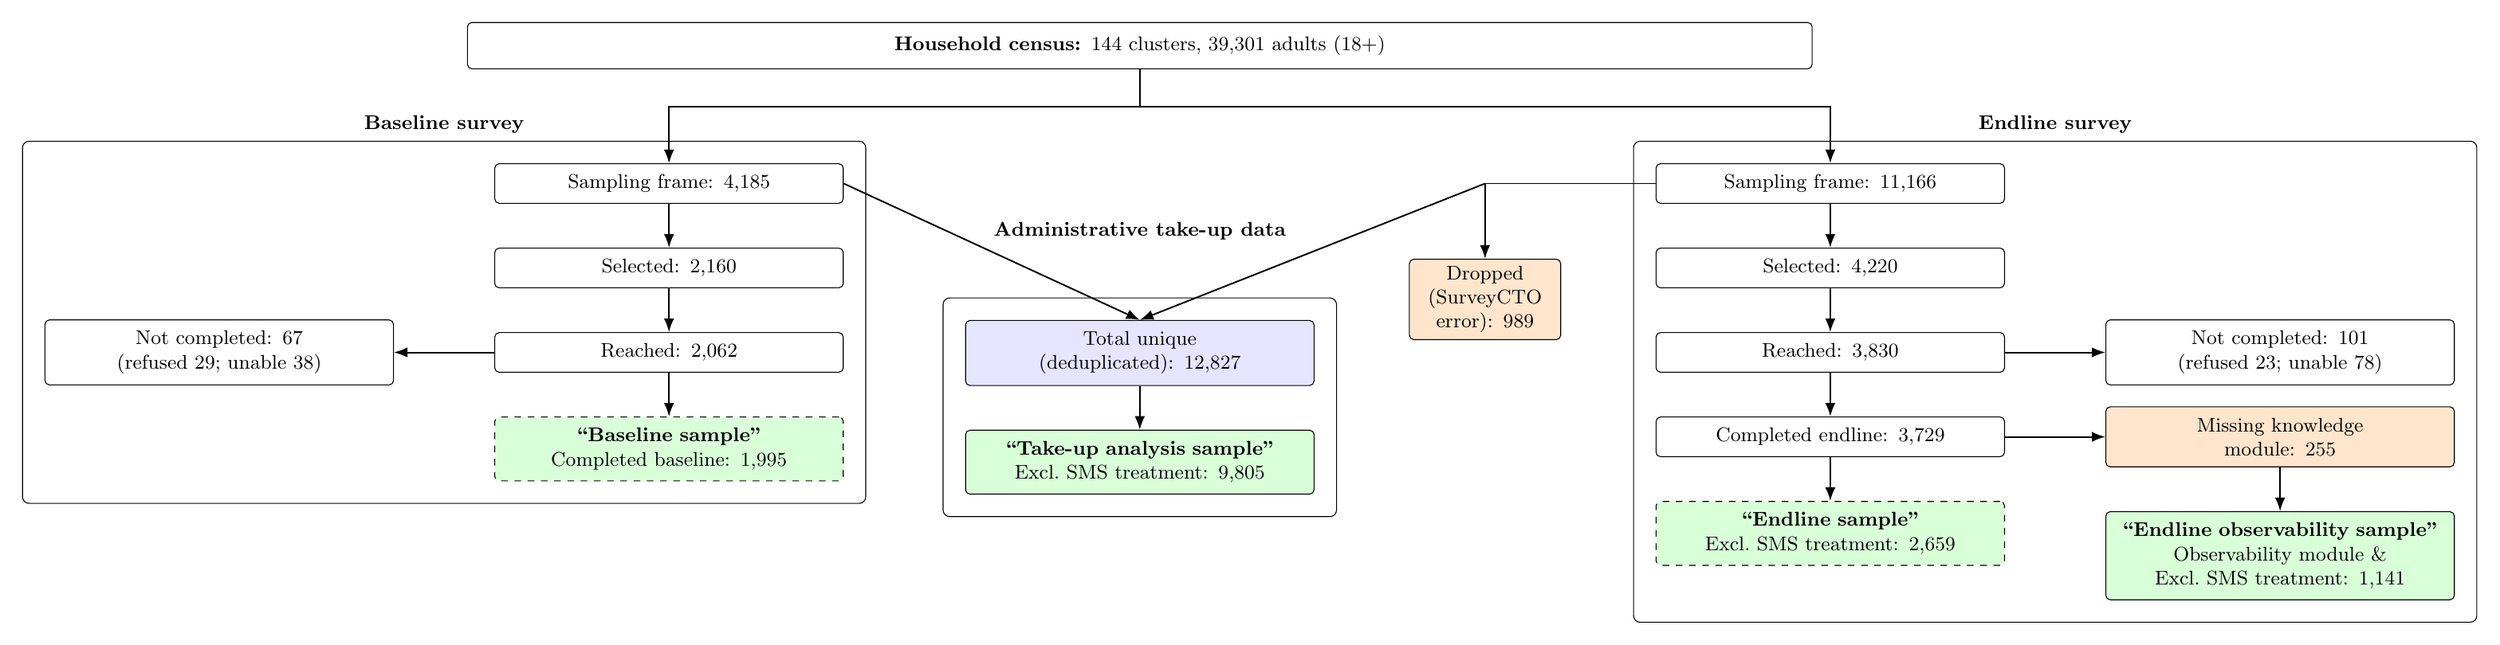
\begin{tikzpicture}[
  node distance = 7mm and 16mm,
  font          = \small,
  %
  % ── Node styles ─────────────────────────────────────────────────
  box/.style      = {draw, rounded corners=2pt, align=center,
                     text width=5.2cm, inner sep=5pt},
  analysis/.style = {box, fill=analysisgreen},
  mon/.style      = {box, fill=monblue},
  issue/.style    = {box, fill=issueorange},
  note/.style     = {box, dashed},
  arrow/.style    = {-Latex, line width=0.7pt},
  darr/.style     = {-Latex, line width=0.7pt, dashed},
  colgroup/.style = {draw, rounded corners=3pt, inner sep=10pt},
]

%% ═══════════════════════════════════════════════════════════════════
%% SHARED TOP — Census frame
%% ═══════════════════════════════════════════════════════════════════

\node[draw, rounded corners=2pt, align=center,
      text width=21cm, inner sep=6pt]
  (census)
  {\textbf{Household census:} 144 clusters,\ 39{,}301 adults (18+)};

%% ═══════════════════════════════════════════════════════════════════
%% COLUMN A — Baseline
%%   xshift = -6.5 cm keeps this column on the left
%% ═══════════════════════════════════════════════════════════════════

\node[box, below=15mm of census, anchor=north, xshift=-7.5cm]
  (bl-sel)
  {Sampling frame: 4{,}185};

\node[box, below=of bl-sel] (bl-tgt)
  {Selected: 2{,}160};

\node[box, below=of bl-tgt] (bl-reach)
  {Reached: 2{,}062};

\node[analysis, dashed, below=of bl-reach] (bl-comp)
  {\textbf{``Baseline sample''}\\
  Completed baseline: 1{,}995};

%% Side branch: not completed (exits left from Reached)
\node[box, left=16mm of bl-reach, anchor=east] (bl-nc)
  {Not completed: 67\\(refused 29; unable 38)};

%% ── Arrows ───────────────────────────────────────────────────────
\draw[arrow] (census.south) -- ++(0,-6mm) -| (bl-sel.north);
\draw[arrow] (bl-sel)   -- (bl-tgt);
\draw[arrow] (bl-tgt)   -- (bl-reach);
\draw[arrow] (bl-reach) -- (bl-comp);
\draw[arrow] (bl-reach.west) -- (bl-nc.east);

%% ── Column A group box ───────────────────────────────────────────
\node[colgroup,
      fit=(bl-sel)(bl-tgt)(bl-reach)(bl-comp)(bl-nc),
      label={[font=\small\bfseries]above:Baseline survey}] {};

%% ═══════════════════════════════════════════════════════════════════
%% COLUMN B — Monitored sample
%%   xshift = 0 cm (center)
%% ═══════════════════════════════════════════════════════════════════

% Merged totals (fed from bl-sel in A and el-frame in C)
\node[mon, below=40mm of census, anchor=north] (mon-uniq)
  {Total unique\\(deduplicated): 12{,}827};

\node[analysis, below=of mon-uniq] (mon-ana)
  {\textbf{``Take-up analysis sample''}\\
  Excl.\ SMS treatment: 9{,}805};
  % {Excl. SMS treatment: 9{,}805\\(\emph{``Take-up analysis sample''})};

%% ── Arrows ───────────────────────────────────────────────────────
% Baseline roster enters from col A
\draw[arrow] (bl-sel.east) -- (mon-uniq.north);

\draw[arrow] (mon-uniq) -- (mon-ana);

%% ── Column B group box ───────────────────────────────────────────
\node[colgroup,
      fit=(mon-uniq)(mon-ana),
      label={[font=\small\bfseries, yshift=8mm]above:Administrative take-up data}] {};

%% ═══════════════════════════════════════════════════════════════════
%% COLUMN C — Endline
%%   xshift = 6.5 cm keeps this column on the right
%% ═══════════════════════════════════════════════════════════════════

\node[box, below=15mm of census, anchor=north, xshift=11cm]
  (el-frame)
  {Sampling frame: 11{,}166};

\node[box, below=of el-frame] (el-sel)
  {Selected: 4{,}220};

\node[box, below=of el-sel] (el-reach)
  {Reached: 3{,}830};

\node[box, below=of el-reach] (el-comp)
  {Completed endline: 3{,}729};

\node[analysis, dashed, below=of el-comp] (el-comp-nosms)
  {\textbf{``Endline sample''}\\
  Excl.\ SMS treatment: 2{,}659};
  % {Excl.\ SMS treatment: 2{,}659\\(\emph{``Endline sample''})};

%% Side branch: not completed (exits right from Reached)
\node[box, right=16mm of el-reach, anchor=west] (el-nc)
  {Not completed: 101\\(refused 23; unable 78)};

%% Side branch: missing knowledge module
\node[issue, right=16mm of el-comp, anchor=west] (el-miss)
  {Missing knowledge\\module: 255};

%% Node below missing knowledge module
\node[analysis, below=of el-miss] (el-know)
  {\textbf{``Endline observability sample''}\\
  Observability module \& Excl.\ SMS treatment: 1{,}141
  };
  % {1{,}141 individuals};


%% ── Arrows ───────────────────────────────────────────────────────
\draw[arrow] (census.south) -- ++(0,-6mm) -| (el-frame.north);
\draw[arrow] (el-frame) -- (el-sel);
\draw[arrow] (el-sel)   -- (el-reach);
\draw[arrow] (el-reach) -- (el-comp);
\draw[arrow] (el-reach.east) -- (el-nc.west);
\draw[arrow] (el-comp)  -- (el-comp-nosms);
\draw[arrow] (el-comp.east) -- (el-miss.west);
\draw[arrow] (el-miss) -- (el-know);

%% ── Column C group box ───────────────────────────────────────────
\node[colgroup,
      fit=(el-frame)(el-sel)(el-reach)(el-comp)(el-comp-nosms)(el-miss)(el-nc)(el-know),
      label={[font=\small\bfseries]above:Endline survey}] {};

%% ── Cross-column: el-frame forks → Total unique and → Dropped ──
% Split point midway between cols B and C, at el-frame height
\coordinate (el-split) at ($(mon-uniq.north |- el-frame.west) + (5.5cm, 0)$);

% Dropped box hangs below the split point (between cols B and C)
\node[issue, anchor=north,
      text width=2.2cm, inner sep=3pt] (mon-drop)
  at ($(el-split) + (0, -12mm)$)
  {Dropped\\(SurveyCTO error): 989};

% Stem: el-frame → split (no arrowhead)
\draw[line width=0.7pt] (el-frame.west) -- (el-split);
% Branch 1: left-then-down to Total unique
\draw[arrow] (el-split) -- (mon-uniq.north);
% Branch 2: straight down to Dropped
\draw[arrow] (el-split) -- (mon-drop.north);

\end{tikzpicture}
\end{document}